%!TEX root = ../../thesis.tex

\section{Technology}

% There are many popular frameworks and libraries that provide a structure, rules and conventions for implementing websites and web applications. 

No IDEs, tools, not even conventions. Es gibt frameworks die eine architektur für webseiten und web-applikationen vorgeben, aber nichts dergleichen für bibliotheken.

Not for building:
Big JS libraries all do it differently.
Top 3 client side JavaScript repositories (stars) on github
https://github.com/search?l=JavaScript\&q=stars\%3A\%3E1\&s=stars\&type=Repositories
Angular.js: Grunt
d3 Makefile, also ein custom build script welche node packages aufruft
jQuery custom scripts, mit grunt und regex und so

Not for Architecture
Angular custom module system with own conventions
d3 mit nested objects (assoc arrays) und funktionen
jQuery mit .fn
ACE mit Klassen, daraus habe ich gelernt

\section{Ich habe verwendet}

Gulp
requireJs
AMDClean
Uglify

JSLint - Douglas Crockford coding dogmatas / conventions
JSCS - JavaScript style guide checker

~~Livereload~~
PhantomJs
Mocha
Chai

Durch Require und AMDClean schöne arbeitsweise (am ende über bord geworfen) und kleine Dateigröße, wenig overhead.

Automatisierte Client side Tests mit PhantomJs und Mocha/Chai

\subsection{ECMAScript 6} 

ECMAScript 6 offers many features for JavaScript including classes and modules. It is not supported by most browsers yet however there are tools like Babel that can transpile ECMAScript 6 to ECMAScript 5. Babel is already used by popular websites like Netflix for JavaScript libraries and Frameworks like React. 

Type will not use ECMAScript 6 and Babel. Even though its features can support the development with syntactic sugar, most of its features can be approached using JavaScript design patterns. The benefit of not using ECMAScript 6 and transpilers are a smaller file size and more independence from third-party tools.

\section{Coding conventions}

Habe mich größtenteils an Crockfordstyle orientiert, aber die Klassen anders geschrieben. Habe den Stil von ACE editor verwendet, denn der ist gut lesbar. Lesbarkeit war mir wichtiger als Crockford style. Für private Eigenschaften und Methoden habe ich die prefix convention verwedendet.
https://developer.mozilla.org/en-US/Add-ons/SDK/Guides/Contributor\_s\_Guide/Private\_Properties
Sie bewirkt keine echte accessibility restriction, aber es ist eine allgemein anerkannten convention und ist auch viel besser lesbar.


\section{Architecture}

%Modulbasiert?
%Erweiterbarkeit
%Es gibt ein Basisobjekt, das ist die Type "Klasse".
%Darin werden dann die anderen Klassen geschrieben "Type.Caret", "Type.Selection", "Type.Range", ...
%Das hat den Vorteil dass das ganze ge-name-spaced ist, so dass ich keine Konflikte mit Systemnamen habe (Range) (und auch nicht mit anderen Bibliotheken)
%Effektiv gibt es eine (flache) Baumstruktur und so mit Ordnung. Für bestimmte Klassen, "Type.Event.Input", "Type.Input.Filter.X" geht es tiefer.
%Der zweite Grund ist, dass ich somit alle Klassen die ich geschrieben habe für Entwickler sichtbar bereit stelle und nicht implizit und versteckt über irgend nen Quatsch.

%Auch angedacht so wie der CKEditor (?) die komplette funktionalität als Plugins zu schreiben. Im Besten Fall

\subsection{Model--view--controller}

Model--view--controller (MVC) is a common apprach for implementing user interfaces and it can be applied to user interface components too. While this apporach can provide clear responsibilites, the problem is that most components, like the caret or the selection, serve a clear atomic purpose and would need to be broken apart into model, view and controller parts themselves, making the architecture fuzzy and complex instead of simplifying it. Following the MVC architecture, the contents of the editor (the text) can be represented in a model (holding the text data and allowing methods to be performed on) and be rendered with a view (displaying the text in the browser). As discussed in \refsection{sec:api_design}, the library shall leave as much freedom as possible to the developers. In and MVC system like this, the contents of the editor could only be changed though the API, since arbitrarily modifying the HTML of the editor's contents would change the view, but not the model. This would create an artificial bottleneck, which cannot be desired.

%The biggest advantage of this approach would be that an abstract view layer could not only render rich-text as HTML, but also as Markdown or in the Open Document Format (ODF). Atom, Spotify or Wunderlist show that web technologies find their way into desktop. Writing to custom formats 
%While especially the latter is not useful in a browser environment


%Ursprünglich ein MVC konzept geplant mit einem Document Model und verschiedenen Renderern, aber über den haufen geworfen.

%\subsection{Modular programming}

\subsection{Modular and object-oriented programming}
\label{subsec:modular_and_oop}

jQuery and CKEditor demonstrate a software architecture in which a core object mainly provides a system to extend its functionality, but does not offer many methods itself\footnote{CKEditor provides a framework for implementing components for it, but does not offer any rich-text functionality in its core. jQuery provides low-level utility methods for JavaScript.}. The actual functionality of both libraries is implemented through extensions while the libraries are usually bundled with a set of ''core extensions'' that provide basic features. CKEditor makes use of modular programming by implementing a major part of its editor as plugins that communicated via well-defined interfaces. jQuery established a paradigm calling any extension a ''plugin'' but instead of using clearly defined interfaces, developers are encouraged to add arbitrary methods to jQuery's base object, which can then be directly accessed. Extending a base object has many advantages

\begin{enumerate}
\item It provides a namespace for the library
\item It provides a structure for extensions to access each other
\item It approaches modular programming and strong decoupling
\end{enumerate}

Modular programming could create a system in which other developers could exchange any component easily to improve performance or enrich functionality. The disadvantage this apporach would be that the need for well-defined interfaces can diminish flexibility. Formalizing interfaces would create complex structures and could make it harder for other developers to contribute to the library instead of inviting them. jQuery goes the opposite direction and encourages arbitrary extensions. jQuery's approach demonstrates that this flexibility, in practice, can withstand possible conflicts. In turn, the low barrier for extending jQuery has spawned a rich collection of extensions and a big community of developers. While jQuery allows to be extended with complex libraries, it is designed to be extended with simple methods. It is difficult to establish complex interactions between extensions.

% However, the biggest factor in coupling the components would still be that components reference each other, not the underlying structure. 


\paragraph{Constructor Pattern} To close the gap between CKEditor's modular programming approach and jQuery's simple extension paradigms, object-oriented programming (OOP) can be used. JavaScript does not offer classes and classical inheritance, however the same functionality can be achieved using the constructor pattern and prototypal inheritance (see \refsection{sec:oop_class}). Functions following the contructor pattern are often called classes or pseudo-classes. Hereinafter the term classes will be used.

%\begin{lstlisting}[language=JavaScript, caption=Type instantiation, label=lst:type_instantiation]
%// Defines the class and its contructor 
%function Foo() {
%  this.instanceVariable = "bar";
%};
%
%// Defines a method for the class
%Foo.prototype.baz = function() {
%  alert(this.instanceVariable);
%};
%
%// Instantiates the class
%var myFooInstance = new Foo();
%
%// alerts "bar"
%myFooInstance.baz();
%\end{lstlisting}

%In JavaScript the \code{new} operator can be used to create instances of \code{Function} objects. Based on prototypical inheritance each instance will share the same methods and attributes of the function's \code{prototype} property, but can still own instance-specific variables and functions by assiging them to the instance object. 


% maybe explain constructor pattern

\paragraph{Modularized structure} For this library a base class will provide the namespace to be extended with other classes implementing the functionality of this library. A set of core extensions provide all components needed for a rich-text editor. The base class will also provide a constructor that will be the library's entry point for other developers to implement a rich-text editor, but, like CKEditor and jQuery, will implement as little functionality as possible itself. The base class and its extensions will be discussed in detail in the sections \refsection{sec:core} and \refsection{sec:modules}. Implementing the library's extensions as classes has many benefits:

\begin{enumerate}
\item As compared to CKEditor and modular programming, strictly defined interfaces are not a necessity. This can improve flexibility and lower the barrier for other developers to contribute. % Auf Nachteile eingehen?
\item As compared to jQuery, classes can have complex interfaces, which allows rich functionality and possiblities in interoperation.
\item Classes are a proven concept for encapsulating functionality and data, protecting access and structing code as well as making it readable.
\item Through JavaScript's prototypical inheritance, the class can be instantiated as often as desired, but will only be allocated once in the browser's memory. Thereby the performance will be improved.
\item Instance variables still allow to reuse a class in different contexts with different inherent data. %Die instanzvariablem sind meistens nur Pointer auf Instanzen anderer Klassen % * Das ganze ist dadurch sehr schlank
\end{enumerate}

As an alternative apporach, the module pattern can be used, which would also allow namespacing, encapsulation and protected access, but would make an implementation much more complicated and be much less readable.

%namespace vorteile = keine namenskonflikte

% and implement as many components as possible as plugins. In its core, the library could create an environment to allow plugins to register and interact with each other. This would 

\section{Base class}
\label{sec:core}

\subsection{Overview}

The \code{Type} class is the base class (see \refsubsec{subsec:modular_and_oop}) and the starting point for users and developers of the library. It provides 4 purposes:

\begin{enumerate}
\item It can be instantiated and offer a high-level API to manipulate text and perform other rich-text related functions
\item It provides a namespace for all of the library's internal classes
\item As an instance, it exposes references to all instances of the internally used classe
\item It exposes its \code{prototype} as a public shorthand attribute
\end{enumerate}

\subsection{Instantiation and usage}
\label{subsec:instantiation_usage}

To develop an editor with the library, it must be instantiated. As discussed in \refsubsec{subsec:api_design_handling_use_cases}, all of the libary's functionality is encapsuled in a class (\code{Type}) that exposes its features as high-level functions. The \code{Type} class is exposed to the \code{window} namespace and is thereby globally accessible. On instantiation it must be passed an \code{HTMLElement}, which's contents will act as the editor's rich-text content. An optional second parameter can be passed to define settings for the editor's instance.

\begin{lstlisting}[language=JavaScript, caption=Type instantiation, label=lst:type_instantiation]
var element = document.getElementById("myElement");
var editor = new Type(element, { paste: "text" });
\end{lstlisting}

The \code{editor} instance variable now offers methods to format, insert and remove text, manipulate the caret and the selection, dynamically change settings and control undo/redo capabilites as well as trigger clipboard commands. The complete API is listed in Figure ABC. For example, to format the characters 10 to 20 as bold and move the caret behind the formatted text, the following methods need to be executed:

\begin{lstlisting}[language=JavaScript, caption=Example commands to format text, label=lst:type_format_example]
editor.selection(10, 20);
editor.format("<strong />");
editor.caret(20);
\end{lstlisting}

\noindent Although it should be noted that the API allows chaining and the above code can be simplified to a single line.

\begin{lstlisting}[language=JavaScript, caption=Example chaining, label=lst:type_chaining_example]
editor.selection(10, 20).format("<strong />").caret(20);
\end{lstlisting}

With the second optional parameter for \code{Type} settings can be passed to determine the eiditor's behavior. As for the implementation of this thesis two settings are avaialable. One to determine the behavior on paste events, the other to turn off default keyboard shortcuts. A full description can be found in figure ABC. Section \refsection{sec:extensions} discusses how extensions of the library can add further options for their own use.

\subsection{Namespace and references} 
\label{subsec:namespace_and_refs}

%The \code{Type} class creates a namespace providing a structure for other classes used in the library and so that these classes do not pollute the global namespace and avoid possible name conflicts. 
The \code{Type} class creates a namespace for other classes used in the library. In JavaScript, functions are first-class objects, namespaces are objects and any object is a namespace. This way, the \code{Type} \code{Function} object (the class itself) can act as a valid namespace. CKEditor takes the same apporach and attaches each module to the \code{CKEDITOR} base class. Any of the classes listed in \refsection{sec:modules} are attached to the \code{Type} class this way. As an exmple, listing \ref{lst:type_declaration_example} shows the declaration of the \code{Type} base class as well as the declarations of the classes \code{Caret}, \code{Range} and \code{Environment}:

\begin{lstlisting}[language=JavaScript, caption={Declaration of Caret, Range and Environment classes}, label=lst:type_declaration_example]
// Declaration of the Type base class
function Type() {};

// Classes defined within the namespace created by Type
Type.Caret = function () {};
Type.Range = function () {};
Type.Environment = function () {};
\end{lstlisting}

The namespace provides a structure for the classes of the library, prevents the pollution of the global namespace and possible name conflicts. In terms of structure, this does not only encapsulate classes related to the library but also allows nesting. This way sub-namespaces can be created, which is especially important for other developers extending the library. The \code{Type} base class already prepares a sub-namespace \code{Type.Events} for events.

Section \refsection{sec:module_architecture} discusses how Type's classes interact to provide its rich-text functionality. One responsibility of the \code{Type} base class is to instanitate all other classes needed for its API and provide getters to each instance, so that each instance can access the other instantiated classes.

%When \code{Type} gets instantiated it in turn instantiates a set of core classes to provide the functionality for its API. To enable each class to access any of the other instantiated classes, the \code{Type} base class provides getters for any of the instances it uses.

%The \code{Type} class is the starting point for developers to implement rich-text editors and to extend the library itself. The 
%The ''Type'' class is the starting point for developers and the only class that is exposed to the global namespace. It serves 4 Resposibilities:
%\paragraph{Provide a namespace for all other classes} All other classes are declared within the ''Type'' namespace.

\subsection{Exposal of Type's \code{prototype}}
\label{subsec_fn_exposal}

Type's functionality is implemented through classes within its namespace. However, this does not expose its functionality to its instances' API. With the constructor pattern, all methods in the \code{prototype} of the \code{Type} class will be available as instance methods. In a simple approach, the library's API can be implemented directly inside the implementation of the \code{Type} class. This contradicts the modular approach of the implementation. jQuery established an effective principle for extending its API. It exposes the library's \code{prototype} with a shorthand attribute as \code{jQuery.fn}. Other modules can extend the \code{prototype} easily and add methods to the libary's API. Type follows the same principle and exposes its \code{prototype} the same way as \code{Type.fn}. jQuery's \code{prototype}---as well as Type's \code{prototype}---can be extended even without exposing it as an attribute, but apart from providing a more convenient way to do so, primarily, jQuery established a simple and yet powerful paradigm that encourages other developers to extend the library's API.

%\subsection{Extensions}

%As discussed in \refsubsec{subsec:modular_and_oop}, Type's functionality is implemented through classes inside Type's namespace. These classes will be utilized by 

%extending works this way: you write classes and extend stuff within type's namespace and when you did that you can add a function to type's api by extending fn.

%There are generally two types of extensions. On the one hand, there are extensions that extend Type with internal features. The \code{Caret} class for example a class a can offer features for displaying and moving a caret within a text. Other classes, for example the \code{Input} class, can listen for keyboard and mouse events, and use this class to display a caret and make it responsive to input.

%To expose a class to other classes, it should be declared within Type's namespace. That means the \code{Caret} class should be declared as \code{Type.Caret} and the \code{Input} class as \code{Type.Input}. This way both classes are visible to each other without polluting the global namespace and are effectively avoiding possible name conflicts.

%To support a tidy code structure the Type namespace can be nested and implement a hierachical structure. The \code{Type} base class implements the namespace \code{Type.Events} that is reserved for events within the Type ecosystem. Other classes are encouraged to nest within the namespace if it is reasonable.

%The second type of extension extends the public API of the Type library, i.e. adds methods for users of the library\footnote{Programmers implementing an editor with Type, see \refsubsec{subsec:api_design_handling_use_cases}}. jQuery has demonstrated a clever concept for this. It exposes its \code{prototype} with a shorthand attribute named \code{fn} and ecourages developers to extend it. This way developers can easily add methods to the library. Type as intended for developing editors follows the same principle.

%There is a general distinction for modules extending Type's public API (intended for users\footnote{Programmers implementing an editor with Type, see \refsubsec{subsec:api_design_handling_use_cases}} of the library) or extending its internal features (for enabling features for developers of the library and/or ultimatively extending the library's API).



\section{Module architecture}
\label{sec:module_architecture}

As discussed in \refsubsec{subsec:modular_and_oop}, Type's functionality is implemented through classes inside Type's namespace. The classes' functionality will be exposed through the base class' \code{prototype}. This section discusses the architecture and interaction of the classes of this library. The implementations and characteristics of each module will be discussed hereinafter.

When the \code{Type} base class will be instantiated, it in turn instatiates a number of classes passing each instance a reference to itself. As described in \refsubsec{subsec:namespace_and_refs} the base class provides setters for each class instance to allow the instantiated classes to access one another. For its basic functionality, Type instantiates the classes \code{Contents}, \code{Formatting}, \code{Caret}, \code{Selection} and \code{Input}.


\begin{figure}[!htb]
\centering
\makebox[\textwidth]{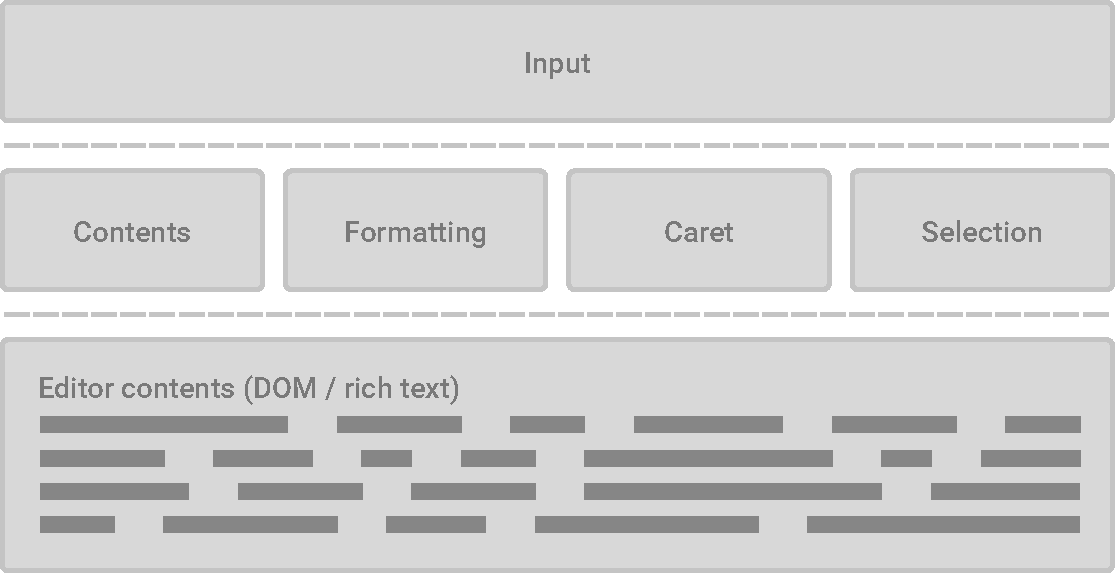
\includegraphics[width=\textwidth]{images/basic-diagram.pdf}}
\caption{Components instantiated by the Type base class}
\label{fig:type_base_components}
\end{figure}

%\begin{itemize}
%\item Contents
%\item Formatting
%\item Caret
%\item Selection
%\item Input
%\end{itemize}

\noindent The \code{Input} class will listen to keyboard input and mouse events. Utilizing the \code{Caret} and \code{Selection} classes it determines which part of the text should be changed or formatted. It passes the formalized edits to the \code{Changes} classes which will record the changes for undo and redo operations. The \code{Contents} class allows adding and removing text and the \code{Formatting} class allows to apply formattings, both using DOM operations. The \code{Changes} class will use these classes to to alter the text according to the change it it should apply.

Usually, text fields contain one caret and display one text selection at a time. This is why the \code{Type} base class instantiate the \code{Caret} and \code{Selection} classes for shared usage within an editor's instance. Of course, this behavior can be extended, for example by instantiating multiple \code{Caret}s for real-time text collaboration.


%\noindent The \code{Contents} and \code{Formatting} classes allow to add and remove text (\code{Contents} class) and to apply text formatting (\code{Formatting} class) to the editor's contents using DOM operations. These classes solely provide functionality. The \code{Input} class will listen to keyboard input and mouse events and utilize the \code{Caret} and \code{Selection} instances to

% apply the input to the appropriate part of the text though the \code{Changes} model. These classes in turn require further classes for their implementation. Section \refsection{sec:modules} will discuss the characteristics of these classes and how they interact. %each class and its specific 


% directed acyclic graph ? 

\section{Type Api}

As discussed in \refsubsec{subsec_fn_exposal}, Type's public API for implementing editors is not hard-coded to the \code{Type} class. Instead it extends \code{Type}'s \code{prototype} dynamically. This conforms the paradigm of having a base class and implementing all its featues in modules. To still ensure maintanability and a clean software structure, the methods for Type's API will not be added arbitrarily by other classes. Instead, all API methods will be implemented by a single module that in turn calls the required methods of the corresponding classes. This allows for a clean and independent software architecture, a separation of concerns and decouples the API from the structure and the implementation of the library.

The module for this, called ''CoreApi'', is the only exception to the rest of Type's implementation in the way that it is not encapsulated in a class. In order to add a method to Type instances, \code{Type.fn} must be extended with a function. This will be done for all methods discussed in \reflisting{lst:rich_text_api}. However this does not require a class contstruct.

Similar to the principles of MVC in which the controllers should be kept small and the implementation should reside in the model layer, the functionality of the API resides in their designated classes, while the API methods are being kept small. The classes are written in a way that allow the API methods to require not more than one function call for their implementation and at most translate their parameters for the class methods.

%\section{Components}
%\label{sec:modules}

%\section{Input}

%82.78\% of internet users support listening to and reading clipboard events. I can support 100\% PROBLEMS
\section{Input reading}

There are various input methods with which users can interact with native inputs. This includes using hardware devices as well as virtual (on screen) devices:

\begin{enumerate} 
\item Hardware keyboard input
\item Virtual keyboard input
\item Mouse (pointer) input
\item Touch input
\item Game controller input (on game consoles)
\item Remote control input (on smart TVs)
\end{enumerate}

When simulating a native input, in a best-case scenario, all these input methods should be accounted for. Fetching input includes two scenarios: The user clicks / touches / or selects the input in any way and does so at any position inside the input. If the user touches / clicks / etc in the middle of the text, the caret should move to that position and typing must be enabled. In environments without hardware keyboards, the libarary must ensure that a virutal keyboards show up. Once the input component is selected, text input must be fetched and written to the editor. There are various options to fetch user input, which will be discussed in the following paragraphs.

\subsection{Events} 

\paragraph{Keyboad} One way to fetch user input is by listening to events. Text input can be read through \texttt{KeyboardEvent}s. Keyboard events will be triggered for virtual keyboards just as for hardware keyboards. When the user presses a key, the event can be stopped and the according characters can be inserted at the position of the caret. As a downside, listeners for keyboard events cannot be bound to a specific element that is not a native text input, that means keyboard events must be listened to on the \texttt{document} level. This not only has (minor) performance downsides but als requires more logic to decide whether a keyboard input should be processed and ultimatively stopped or ignored and allowed to bubble to other event listeners of a website. Furthermore, there can be edge cases, where even though a keyboard event should write contents to the editor, the event itself is supposed to trigger other methods that are not part of the editor. Keyboard events are supported by all major browsers across all devices.

\paragraph{Mouse (pointer) and touch} To support clicking or touching inside the editor's contents \texttt{MouseEvent}s and \texttt{TouchEvent}s can be used. Mouse events are supported on all major desktop browsers and all mobile browsers support touch events. Both event types support reading the coordinates indicating where the click or touch has been performed.

\paragraph{Remote controls} Although some smart TVs offer keyboards, mice, pointers similar to Nintendo's Wii remote, input via smartphone apps and many others, button-based remote controls are offered with almost any smart TV and remain a edge case for interacting with a text editor. In such an enviroment, users commonly switch between elements by selecting focusable elements with a directional pad. Using only events would not account for this case since there would be no focusable element representing the editor. Recent browsers on Samsung's and LG's smart TVs are based on WebKit\footnote{\url{http://www.samsungdforum.com/Devtools/Sdkdownload}, last checked on 07/22/2015} while Sony's TVs use Opera. Before 2012 Samsung's browser was based on Gecko. All of these browsers and browser engines supprt keyboard events to fetch input.

\paragraph{Clipboard} A problem with relying entirely on events is the lack of native clipboard capabilities. Unless a native text input (including elememts with enabled editing mode) is focused, shortcut keys for pasting will not trigger a paste event and the mouse's context menu will not offer an option for pasting. \textit{Recent versions of Chrome, Opera and Android Browser\footnote{\url{http://caniuse.com/\#feat=clipboard}, last checked on 07/22/2015} allow triggering arbitrary paste events on elements in editing mode thereby read the cliboard contents. With this, shortcuts could be enabled with JavaScript and instead of the native context menu, a customly build context menu using HTML could be shown that allows the user to paste, but this only works on elements in editing mode and only in these three browsers.}

\subsection{Hidden native input fields} 

As discussed in \refsection{sec:approaches_for_imitating_native_components}, the source code editors Ace and CodeMirror use a hidden (native) input field to fetch the user's keyboard input. While it appears to the user he or she is entering text in a syntax-highlighted representation of the source code, in reality the user enters his or her text in a hidden \code{textarea} element. The input will be processed and displayed with syntax-highlighting. This solves many problems of relying solely on events

\begin{itemize}
\item The hidden \code{textarea} can be focused with the tab key.
\item The hidden \code{textarea} can be focused with remote controls.
\item Virtual (on screen) keyboards will show up.
\item Keyboard shortcuts for clipboard events work.
\item It can display a native context menu that allows pasting.
\end{itemize}

\paragraph{Implementation} To achieve this, a \code{textarea} must be created when the editor gets instantiated. Since browsers scroll the \code{textarea} into view when it receives the focus, it must be positioned in the visual representation of the editor, so the editor will be scrolled into view. This perfectly mimicks the browser's native behavior. To maintain the illusion that the user acutally writes inside the visual represenation of the editor the \code{textarea} must be hidden.

\paragraph{Focus} Whenever the user clicks inside the editors visible contents, the (fake) caret will be set (see \refsubsec{subsec:caret}) at the according text position. To enable text input, the hidden \code{textarea} will be focused. The \code{textarea} is focusable using the tab key or a remote control on a smart TV. It will also trigger focus and blur events. This way, it is possible to display the caret when the \code{textarea} receives the focus and read its input as well as hiding the caret on blur and thereby perfectly mimick the native behavior for input events.

\paragraph{Virtual (on screen) keyboard support} The \code{textarea} will be focused when the user clicks or touches inside the editor as well as with the tab key and remote controls. Focusing a text input triggers the display of native virtual keyboards.

\paragraph{Pasting} When a the textarea is foucsed, pastiing via keyboard shortcuts is natively available. To enable pasting with the context menu, the \code{textarea} must be moved to the pointer's position on a \code{mousedown} event. Following the order of \code{MouseEvent}s, this will be completed, before the context menu will be triggerd. This way it will be triggered on the \code{textarea} and contain a paste option.

\paragraph{Reading input} \code{textarea} elements support \code{input} events which can be used to read the text entered by the user. The input can be processed as discussed in \refsection{sec:module_architecture} and be removed from the textarea. Input reading requires further processing before it can be passed on to trigger a change in the editor's contents. The specifics on processing the input will be discussed in section \refsection{sec:input_pipeline}.

\section{Input Pipeline}
\label{sec:input_pipeline}

\subsection{Overview} 
\label{subsec:input_pipeline_overview}

\begin{figure}[!htb]
\centering
\makebox[\textwidth]{
\includegraphics[width=\textwidth]{images/input-pipeline.pdf}}
\caption{Input pipeline with sample filters}
\label{fig:type_base_components}
\end{figure}

Before the text read from the hidden \code{textarea} will be passed on to the \code{Changes} class, it will be passed though a series of \code{Filter}s, called the ''input pipeline''. The input pipeline has 3 basic responsibilites.

\begin{itemize}
\item Stop and dispatch input that that shoud trigger functions of the library
\item Implement rich-text editing behavior
\item Filter and transform input
\end{itemize}

The input pipeline is part of the \code{Input} class. The pipeline itself is an array of input filters that can be added, removed and orderd with a designated API.

JavaScript does not support the concept of \code{Interfaces} and although the constructor pattern allows class-like structures, it does not support classical inheritance. Both can be implemented through supporting constructs and the \code{Utilities} class (see \refsection{sec:utilities_class}) implements a method for the latter. \textit{REWRITE CORRECT} Instead, each input filter registers and specifies for which input should be called. For instance, a filter can register to be called when the user presses the \keystroke{ctrl}\keystroke{s} key combination and trigger a ''save'' function. The input is passed to the filters as an event that can be stopped from bubbling. This way it can be prevented that pressing \keystroke{ctrl}\keystroke{s} will also insert an ''s'' character to the editor. The order in which filters will be called is important. Some filters process the input and must cancel the event not only to prevent a character to be inserted, but also to prevent other filters from taking action.

%    unless implemented with supporting constructs\footnote{Interfaces can be implemented though helper classes too}. These constructs can be costly in terms of file size and performance. For this reason, input filters do not implement a formalized interface and do not inherit a base filter class. 

The basic filters implemented for this library will be listed hereinafter, grouped by the responsibility as listed above.


%The \code{Input} class will pass any entry made in the \code{textarea}

%The \code{Input} module checks .
%Filters are classes that can be instantited and added to the 

% The order in which filters will be applied can be important

\subsection{Triggering functions}

\paragraph{Caret} Commonly, when a user presses one of the arrow keys inside a text, the caret will be moved and of course, in a browser eivironment, this is not different. To mimick this behavior arrow key input will be intercepted by the \code{Caret} input filter class, which will move the caret that has been instantiated by the \code{Type} base class (see \refsection{sec:module_architecture}). It will also account for modifier keys and the operating system used and move the caret accordingly.


\paragraph{Command} The \code{Command} input filter class checks for and intercepts keyboard shortcuts commonly used for text formatting. 

\begin{itemize}
\item \keystroke{ctrl}\keystroke{b} Formats the currently selected text bold.
\item \keystroke{ctrl}\keystroke{i} Formats the currently selected text italic. 
\item \keystroke{ctrl}\keystroke{u} Formats the currently selected text underlined.
\end{itemize}

To format the text, by default, the tags \code{strong}, \code{i} and \code{u} will be used. Since in some cases this might not be desired, these default keyboard shortcuts can be turned off by setting the according options (see \refsubsec{subsec:instantiation_usage}).

The input event implements an abstraction to either check for the \keystroke{ctrl} key or the \keystroke{cmd} key depending on the operating system of the user (see \refsection{sec:events}) so that the abovementioned shortcuts can (only) be triggered with the \keystroke{cmd} key instead of the \keystroke{ctrl} key on the OS X systems.


\subsection{Rich-text behavior}

As discussed in \refsubsec{subsec:concept_native_imitation}, most rich-text editors support the user with a common behavior depending on the user's input. This behavior can be abstracted in a simple way using the input pipeline. The following paragraphs describe the rules and filters implemented by default. Further rules can easily implemented as input filter and being added to the input pipeline.

\paragraph{Headlines} When a user presses \keystroke{enter} while the caret is located at the end of a headline, a new text paragraph will be created behind the headline and the caret will be placed inside it.

\paragraph{Lists} Pressing \keystroke{enter} inside a list item creates a new list item behind the current one and the caret weill be placed inside it.

\subsection{Filterring and transformation}

\paragraph{Line Breaks} To display a line break in the visible rich text (i.e. the markup) a \code{br} or \code{p} tag must be inserted\footnote{To enforce a line break other tags. like the \code{div} tag can be used, but would not be semantically appropriate in this context}. When the user presses the \keystroke{enter} key it does not suffice to insert a carriage return and/or line feed. This input will be intercepted and instead a \code{br} tag will be inserted to the editor's contents. As discussed in \refsubsec{subsec:input_pipeline_overview}, it is important that this filter will be invoked after the \code{Headlines} and \code{Lists} filters, so they can apply their behavior and prevent this filter's behavior.

\paragraph{Remove} To delete text from the editor the \code{Remove} filter checks for \keystroke{backspace} and \keystroke{del} key inputs. Depending on whether there is a text selection or not, it either deltes the selection's contents or one character left/right of the caret.

\paragraph{Spaces} Browsers display adjacent spaces as a single space. This is an unusual behavoir for text editing. The \code{Spaces} input filter checks if adjacent spaces are being entered and inserts non-breaking spaces.

\subsection{Events} As an alternative apporach, for every input that the user makes, an event could be triggered. Input filters could be implemented as event handlers. With this, the same functionality could be achived without an input pipeline. A designated pipeline however provides a clearer mental model for processing the input, it allows a separation of concerns. An input filter has a specific purpose and context as compared to an arbitrary input event handler. It can also be made sure that any input filter will be run before triggering an input event. This way input event handlers only receive actual text input for the editors contents while keyboard shortcuts and other keypresses have been filtered out.

\subsection{Extendability} The input pipeline is intended to be extended. It serves as an entry point for other developers to process input. For this, the \code{Input} class provides an API to add, remove and reorder input filters.

%While these are the basic responsibilites 


%pipeline idea
%rules for behaviours (lists, headlines, enter, spaces...)
%Ursprünglich so gedacht: Was gehört zu einem editor X, Y und Behaviour. Für Behaviour aber das input pipeline system gefunden, welches das ganze schön abbildet/löst.
%Noch mal skimmen und sehen ob da was dabei ist, besonders "Detour": http://marijnhaverbeke.nl/blog/browser-input-reading.html

\section{Pasting}



Kontrolle durch die Implementierung mit einem versteckten Eingabefeld. Erst mal gibt es ein reliable Paste event, was es in keinem Editor basierend auf contentEditable gibt. 2. Hat man volle Kontrolle über den Inhalt, was gepastet wird und was nicht. Und das ganze mit einer einfachen API. Pasting sollte internes event ausloesen.

% Apart from rich-text editors there are also third-party JavaScript libraries that allow embedding code editors with syntax highlighting in a website. The ''Ajax.org Cloud9 Editor (Ace)'' and ''CodeMirror'' editor are amongst the most well-known choices. Both editors keep an internal representation of the plain-text (i.e. non-highlighted) contents of the editor, parse it and display a highlighted version using HTML in a designated \texttt{div}. Both editors use a hidden \texttt{textarea} in which the user enters his or her input. The input will be read from the \texttt{textarea} and

% which is presented to the user as the input field.

\section{Caret}
\label{subsec:caret}

The \code{Caret} class provides all functionality to place and move a caret in a text. It provides methods to be moved left, right, up and down in a text as well as to be placed at at specific position in a text. The visual representaion of the caret is a \code{div} element, styled to imitate a text caret. Using a CSS3 animation, it imitates the ''blinking'' common for native text carets. The challenge with this class is that it must be able to be moved within text and in any kind of formatting, split up into any combination of DOM nodes. In terms of text and text formatting, it must account for that

\begin{enumerate}
\item Letters have different widths and heights
\item Different fonts have different letter dimensions
\item Different formattings like a headline, italicised text or text with a specifically set font size, result in different letter dimensions
\end{enumerate}

\code{CodeMirror} solves these problems by measuring each letter with the use of text ranges. The \code{Range} interface offers methods to be spanned over a specific text and to read the range's offsets. These methods can be used to span a range over a single character, read its offsets and place the caret next to it and giving it the same height as the character.

To move the caret left or right, the according characters left and right of its current offset will be measured using this method. To move it up and down across text lines, the caret must check the offsets of every character, starting from the character of the current offset, until it reaches the character above or below it that is closest to its horizontal position. As discussed in section \refsection{sec:cache}, a cache for this cannot be applied. The complexity of this is $O(n)$, however in practice, the number if characters this will affect is limited by readability and usability of the text editor. Mobile devices, that generally have less performance than desktop machines, have smallers screens displaying less characters per line. While this is not necessarily the case, it can be expected by good software design.



\subsection{BiDi support}
\subsection{IME} 
http://marijnhaverbeke.nl/blog/browser-input-reading.html 
https://en.wikipedia.org/wiki/Input\_method

\section{Range}

The \code{Range} class is a utility class and an abstraction for the native \code{Range} interface. The native implementation is prone to bugs on many browsers. As discussed in \refsection{sec:interaction_with_browser_apis}, instead of fixing the API by shimming its methods, the \code{Range} class implements all methods related to ranges while trying to interact as little as possible with the native API. On top of the methods required by Type that are implemented by the native \code{Range} interface, this class implements additional methods specific to the API.

%CodeMirror uses (native) \code{Range}s for text

%Ranges are specifically used to 

%Ranges are mainly used by the implementations of the caret and the selection.






\section{Selection}
Fake damit copy \& past nativ funktioniert
Obwohl eine selection mehrere Ranges haben kann, wird das von keinem Browser unterstützt http://stackoverflow.com/questions/4777860/highlight-select-multiple-divs-with-ranges-w-contenteditable/4780571\#4780571
Habe versucht mit die Darstellung über getClientRects zu emulierten, aber das ist buggy siehe https://github.com/edg2s/rangefix/blob/master/rangefix.js


\paragraph{Selection Overlay}
overlay

\section{Formatting}
formatting

\section{Change Listener}
change

\section{Contents}
contents

\section{Development}

The \code{Development} class is intended to contain utility methods to support the development of the library. As for the development of this thesis, it was sufficient to implement logging methods.

\section{Dom Utilities}

The \code{DomUtilities} class encapsulates common methods for all DOM operations other than traversal. It has no inherent purpose but many other classes perform the same DOM operations, which hence reside in a common library to avoid code duplication.

\section{Dom Walker}

Working with text implies having to traverse the DOM, i.e. the nodes inside the text often. The {DomWalker} utility class solves this problem. The DOM API offers methods to access a node's siblings, children and parents, but it must always accounted for cases when any of these is \code{null} (there is no parent, sibling or child) or when they overflow the bounds of the editor's contents. But more importantly, for text editing, it is usually necessary to access the next (or previous) node in the document's content flow which can either be the parent, sibling or child. Also, it is often the case that it is not only necessary to fetch the next node, but to apply a filter to only fetch a specfic node, for instance a text node or only a text node that has contents visible to the user\footnote{Any text node consisting of whitespace only will not be displayed by any major browser}. Browsers offer a native API for this, called \code{TreeWalker}, but it is said to be slow\footnote{\url{http://jsperf.com/qsa-vs-node-iterator}}, is only partially supported by Internet Explorer 9\footnote{\url{https://developer.mozilla.org/en-US/docs/Web/API/NodeIterator\#Browser_compatibility}} and has been critisized for its verbose API\footnote{By John Resig, author of jQuery\url{http://ejohn.org/blog/unimpressed-by-nodeiterator/}}.

\subsection{API}

The \code{DomWalker} class offers high-level methods for traversal, designed to quickly apply the most common filters. I can be instantiated with multiple shorthand parameters.

\begin{algorithm}
\caption{Simplified text formatting pseudocode}
\label{alg:format_pseudocode}
\begin{algorithmic}[1]
\State new DomWalker(startNode, node);
\State new DomWalker(startNode, 'filtername');
\State new DomWalker(startNode, filterFunction()\{\});
\State new DomWalker(startNode,\{optionsObject\});
\end{algorithmic}
\end{algorithm}

\noindent The API is not only designed for the development of this library but most importantly to be a utility too for developers extending the library or implementing editors.

%The API is designed for an easy and high-level usage to simplify the workflow for developing the library, but most importantly to offer a high-level and easy-to-use concept to other developers.

%dom walker. Used SO OFTEN in the project. Goal is to have a really simple api new DomWalker('text') by having lots of pre-defined magick in it.

\section{Environment}

The \code{Environment} class checks and provides informations on the current browser environment and its features. This class is especially important to mimick native behavior for user interaction. For instance, depending on the operating system, either the control key or the command key should be used to implemnt keyboard shortcuts. To check for specific feature support, it is favourable to use duck typing within each class.


\section{Events}
\label{sec:events}
\subsection{Overview}

It is possible to trigger custom (native) events using the \code{CustomEvent} interface on modern browsers \textit{todo explain browser support}\footnote{\url{https://developer.mozilla.org/en/docs/Web/API/CustomEvent\#Browser_compatibility}}. Internet Explorer 9 and below allow this through similar interfaces. This system could be use for triggering events for components of Type. However, this would trigger events that that are only relevant within the library in the global namespace. To avoid this, Type implements its own event system that populates events only within the library. Events from within the editor that can be useful to the website or web application Type is used in should still be triggered as native events in the browser's global namespace. During the development of the library no such even has (yet) occured.

%Dazu entscheiden dass es ein Type-Internes Eventsystem gibt, dessen Events nur in Type existieren. Damit polluten die nicht den globalen (name)space mit events. Nur bestimmte events werden global (nativ) getriggert, und das sind genau die events, die nach aussenhin von Belang sind und abgegriffen werden koennen sollen (=API design)

\subsection{Event Api}

The \code{EventApi} class provides an API to add and remove event listeners as well as to trigger events. It provides instance and static methods.

\begin{lstlisting}[language=JavaScript, caption={EventApi methods}, label=lst:eventapi_methods]
// Static methods
EventApi.on(eventName, eventHandler);
EventApi.off(eventName, eventHandler);
EventApi.trigger(eventName, eventObject);

// Instance methods
EventApi.prototype.on(eventName, eventHandler);
EventApi.prototype.off(eventName, eventHandler);
EventApi.prototype.trigger(eventName, eventObject);
\end{lstlisting}

%\begin{itemize}
%\item \code{trigger} 
%\item \code{on}
%\item \code{off} 
%\end{itemize}

Using the \code{Oop} class (see \refsection{sec:oop_class}), these methods will be inherited by the \code{Type} class. This way, using the \code{trigger} method, events can be triggered within the scope of a \code{Type} instance and be captured using the  the \code{on} method. Event handlers can be removed using \code{off} method.

The static methods will also be inherited by the \code{Type} class. This is necessary to trigger events that are \textit{Type} specific but not \textit{instance} specific. Most importantly a ''ready'' event will be triggered on every instantiation of the \code{Type} class. This way plugins and other third-party scripts can run initialization scripts.

The first parameter for any of these methods is always the event name that should be listened to, stopped to be listened to or triggered. The second parameter of the \code{trigger} method is an event object that can be an instance of any of the classes discussed in sections \refsubsec{subsec:type_event} through \refsubsec{subsec:paste_event}. The second parameter of the \code{on} and \code{off} methods can be a \code{Function} that will receive the object, that has been passed to the trigger method, as first parameter.

Plugins and third-party libraries can trigger arbitrary event names and pass arbitrary data. As a paradigm and in terms of a \textit{good programming style}, event objects should be passed. Event objects are inherited from the \code{TypeEvent} or conform its API.

\subsection{TypeEvent}
\label{subsec:type_event}

\begin{lstlisting}[language=JavaScript, caption={TypeEvent API}, label=lst:eventapi_methods]
TypeEvent.data([options]);
TypeEvent.cancel();
\end{lstlisting}

The \code{TypeEvent} is a generic, general-purpose event. It can store arbitrary data and offers an API to be stopped from bubbling. A full API description can be found in Listing XY.

\subsection{InputEvent}
\label{subsec:input_event}

The Input \code{InputEvent} will be triggered by the \code{Input} class after a keyboard input has passed the input pipeline. It inherits all methods from the \code{TypeEvent} to conform the event system and contains information on the key and the modifier keys pressed. The key is represented with its key code and the keyname. They keyname will be mapped from the keycode and is represented by a list of many readable names including ''backspace'', ''enter'', ''space'', all letters and many others. The list not complete but can be extended during further development. The modifier keys include ''shift'', ''alt'', ''ctrl'' and ''meta''. ''meta'' is the browser's name for the \keystroke{cmd} key on OS X systems. OS X uses the \keystroke{cmd} key as modifier the same way Windows and Linux use the \keystroke{ctrl} key. To support implementing for both platforms the ''cmd'' modifier will be set when a user holds the \keystroke{cmd} key on OS X \textit{or} the \keystroke{ctrl} key on other platforms.

\subsection{PasteEvent}
\label{subsec:paste_event}

The \code{PasteEvent} will be triggered when the user pastes contents from the clipboard \textit{before} it will be inserted to the editor's contents. It contains the clipboards contents and can be cancelled so that other developers are free to manipulate and stop a paste event.


%\section{Plugin Api}
%plugin api
\section{Settings}

Settings

\section{Text Walker}

The \code{TextWalker} class acts as a container for all functions related to measuring text offsets. It provides utility methods to determine the character offset from one text node to another or, vice versa, which text node can be found at a text offset, starting from another given node. Both methods are required by various classes and are thus, centralised. 


\section{OOP}
\label{sec:oop_class}

The \code{Oop} class implements a simple approach to extend the contructor pattern with basic classical inheritance. It does so by providing an \code{inherits} method, that copies all methods and attributes from one prototype of a class to another. In this simplified apporach, parent methods cannot be called from child classes with a unique keyword (like ''super'') as it is the case with Java or other languages using classical inheritance.

Any static methods and attributes of a class will also be inherited by coping any method and variable defined on the \code{Function} object passed.


\section{Utilities}
\label{sec:utilities_class}
The \code{Utilities} class is a general-purpose class that contains methods to extend JavaScript's features. It contains methods to work with data structures and to detect object types.

\section{Cache}
\label{sec:cache}

For traversing the text, for example when the caret moves, the text will need to be measured. All measurements can be stored to a cache to only perform the same measurement operations once. On the other hand, the library should be a ''good citizen'' on a website, which means it should be as unobtrusive and leave the developers as much freedom as possible. The library will essentially modify parts of the DOM that act as the editor's contents. It should be agnostic to the editor's contents at all times to give other developers the freedom to change the contents in any way needed without breaking the editor. A cache must account for external changes. The DOM3 Events specification\footnote{\url{http://www.w3.org/TR/DOM-Level-3-Events/}, last checked on 07/21/2015} offers \texttt{MutationObserver}s to check for DOM changes. This feature is not supported by Internet Explorer version 10 or less\footnote{\url{http://caniuse.com/\#search=mutation}, last checked on 07/21/2015}. Internet Explorer 9 and 10 offer an implementation for \texttt{MutationEvent}s\footnote{\url{http://help.dottoro.com/ljfvvdnm.php\#additionalEvents }, last checked on 07/21/2015}. The W3C states that ''The MutationEvent interface [...] has not yet been completely and interoperably implemented across user agents. In addition, there have been critiques that the interface, as designed, introduces a performance and implementation challenge.''\footnote{\url{http://www.w3.org/TR/DOM-Level-3-Events/\#legacy-mutationevent-events}, last checked on 07/21/2015}. Apart from that, the benefits of a cache may not signifcantly increase the library's performance. The actions that can be supported by a cache, most importantly moving the caret in the text, are not very complex and do not noticably afflict the CPU. Implementing an editor that is stateless in regards of its contents can also improve stability.


\section{Real-time collaboration with Etherpad} 

\subsection{Overview}

To achieve real-time collaboration with multiple type editors, Etherpad\footnote{Etherpad has been completely rewritten under the name Etherpad Lite. However, its official website no longer links to its former source code. For simplicity, the name Etherpad will be used, referring to its rewrite as Etherpad Lite} can be used. Etherpad is a web-based collaborative real-time text editor with rich-text capabilites. It provides a server, written in JavaScript using Node.js as well as a web-based rich-text editor. Both components are distributed in one package and are meant to be used together.

To achieve real-time rich-text collaboration, multiple web-based clients communicate with a server via WebSockets using socket.io. Each client owns a local version of the document that it needs to sync with the server. The server uses an operational transformation algorithm to merge each change to the document accounting for all changes and then urges each client to update their local contents according to the final document.

\subsection{Changesets}

For this, Etherpad uses the concept of so-called ''changesets''. Each client sends its local changes, debounced to an interval of 500 milliseconds, as a serialized string---the changeset---to the server. The changeset includes all text insertions, removals and formattings of the last time frame. Along with the changeset, it sends a document revision number that the changeset is based on to the server. The document revision number increases with every changeset that has been accepted and applied to the document on the server side. The document on ther server side is saved as a stack of changesets, which ultimatively form the current document. For performance reasons, snapshots can be taken that save the document as formatted text. 

Based on the revision number that the client provides with the changeset, the server can apply it to the version of the document the client was working on. The server will apply the resulting changes to all newer revisions of the document (if present) and send a changeset and the latest revision number back to the client.

The changeset it sends back includes the differences from the the client's current revision of the document (with its own changes already applied) to the the latest revision on the server that includes the result of all changes the server had to perfom along each revision as just described.

As a last step, the client must apply the changeset it got from the server to its local document to display the most recent version to the user and update its local revision number to what it got from the server.

\subsection{Merging}

In a collaborative environment, it can happen that two (or more) clients send different changesets to the server that are based on the same document revision. It is the responsibility of the server to merge both changes so that it preserves either intend. As explained in the ''Etherpad and EasySync Technical Manual''[citation needed], to solve this, for a document $X$ with the conflicting changesets $A$ and $B$, the server computes the new changesets $A'$ and $B'$ such that
$$XAB' = XBA' = Xm(A,B)$$
where $Xm(A,B)$ is the merge of $A$ and $B$ applied to the document $X$. The changesets $A'$ and $B'$ will be sent to the respective clients, which will apply it to their local documents to sync with the document on the server. To compute a changeset $A'$

\begin{itemize}
\item Insertions in $B$ become retained characters in $A'$
\item Insertions in $A$ stay insertions in $A'$
\item Retain whatever characters are retained in \emph{both} $A$ and $B$
\end{itemize}

For $B'$ this applies vice versa. This implies that anything affected by the changesets and is not inserted or retained will be removed. \textit{// CHECK ON THIS AGAIN!}

\subsection{Etherpad Client implementation}

Clients interact with the server via WebSockets using socket.io. To sync their own changes with other clients, a client does 4 things.

\begin{itemize}
\item Request a the full document from the server
\item Send a changeset to the server
\item Receive acknowledgement from the server for a submitted changeset
\item Receive a changeset from the server submitted by another client
\end{itemize}

\noindent When Etherpad's client connects to the server it receives an initial snapshot of the entire document as a string. To submit changes, the client uses a three-step architecture. Any local changes that have not been sent to the server yet, the client stores in a changeset $Y$. Any changeset sent to the server must be acknowledged by the server as it has applied  the changeset to its document. Any changeset that has been sent and not been acknowledged yet will be stored in a as the changeset $X$. The document as it is acknowledged by the server is stored in a changeset $A$. The document visible to the users can be expressed by the represention of $A \cdot X \cdot Y$, i.e. applying each changeset to the next.

Whenever a user applies a local change, the changeset $Y$ will be updated. Every 500 milliseconds, but not before a changeset submitted to the server as been acknowledged, the changeset $Y$ will be sent to the server and $Y$ will be assigned to $X$. $Y$ will be set to a changeset that contains no changes. When the client hears the acknowledgement for $X$ from the server, $X$ will be applied the changeset $A$ and $X$ will be set to contain no changes.

This architecture supports receiving changesets from other clients as they must be applied to a client's local changes, committed and uncommited, as well as the document version as acknowledged by the server. When a client receives another client's changeset $B$ it will perform 4 steps.

\begin{enumerate}
\item Compute a new changeset by merging $Y (X \cdot B)$ and apply it to the document visible to the user.
\item Apply $B$ to $A$.
\item Compute a new changeset by merging $B$ and $X$ and assign it to $X$
\item Compute a new changeset by merging $(X \cdot B) \cdot Y$ and assign it to $Y$
\end{enumerate}

The operations needed to merge the changesets on the client, are the same operations for merging changesets on the server.

\subsection{Type Client implementation}

Etherpad's technology can be used to enable real-time collaboration for Type. While Etherpad offers a web-based client, its imeplementation has three flaws:

\begin{enumerate}
\item It cannot be integrated easily in other web applications.
\item It does not generate semantic markup. It is cluttered with control sequences.
\item It's hard to extend.
\end{enumerate}

Etherpad does not provide a documentation on its client--server protocol, but it can be reverse engineered. It is possible for third-party libraries to communicate with an Etherpad server alongside Etherpad's ''native'' clients, as long as a third-party library (like Type) conforms the protocol.

Etherpad's collaboartion functionality comes with a cost in file size and may only be used in specific use cases. This is why this feature is implemented as an optional extemsion (compare \refsection{sec:extensions}) in a separate file. To enable collaboration the designated JavaScript file needs to be added to the website.

\begin{lstlisting}[language=html, caption=Enabling real-time collaboration to Type, label=lst:add_etherpad_html]
<script src="type.js"></script>
<script src="type.etherpad.js"></script>
\end{lstlisting}

\code{type.etherpad.js} adds the classes it requires to the \code{Type} namespace and add a static constructor to the Type library:

\begin{lstlisting}[language=JavaScript, caption=Factory method to generate a collaborative Type instance, label=lst:etherpad_constructor]
var element = document.getElementById("myElement");
var editor = Type.fromEtherpad(element, "http://example.com/editor/myEditorId");
\end{lstlisting}

The constructor used in line 2 of \reflisting{lst:etherpad_constructor} will connect to an Etherpad server and load the contents of a document and append it to the element given as first argument.

Will use the change listener to watch changes. Has an own class to serialize changesets. One class for pushing changes to the server. Uses caret class to display other collaborators. And has a class to apply incoming changes.

This architecture provides an unobtrusive way to integrate real-time collaboration in the Type library. It does not depend on a specific implementation of an editor. Developers are free to implement any editor specific to their needs with integrated real-time collaboration.

% Collaboration with etherpad ist wirklich einfach zu machen mit meinem coolen editor. Mein Editor ist ganz ganz toll dass das so einfach geht, ja!



\section{Extending}
\label{sec:extensions}

\subsection{Overview}

Type's modular structure is designed for extension. Type's \code{prototype} has been exposed as \code{Type.fn} and all its classes in the \code{Type} namespace. This provides other developers with all of Type's functionality in a sctructured and accessible manner. Type is designed to lower the barrier for and encourage developers to extend Type by giving freedom and possiblities in how to implement an extension and trying to avoid compulsorily use of interfaces or configurations.

jQuery demonstrates a liberal apporach for writing extensions and experience shows that name comflicts are minimal and ''good'' extensions are naturally favored over ''bad'' extensions by the community of web developers.

\subsection{API extension}

\begin{lstlisting}[language=JavaScript, caption=Example Type API extension, label=lst:api_extension_example]
Type.fn.myMethod = function () {};
\end{lstlisting}

As discussed in \refsubsec{subsec_fn_exposal}, to add a method to Type's public API, its base class' prototye can be extended with a function using the \code{Type.fn} shorthand attribute. Static constructors can be added by extending the \code{Type} \code{Function} object.

\begin{lstlisting}[language=JavaScript, caption=Example custom static constructor, label=lst:example_static_constructor_extension]
Type.myConstructor = function () {
  return new Type();
};
\end{lstlisting}

\subsection{Namespace extension}

As discussed in \refsubsec{subsec:namespace_and_refs}, to implement extensions for Type, the \code{Type} namespace can be used to add custom classes or sub-namespaces.

\begin{lstlisting}[language=JavaScript, caption=Example Type namespace extension and usage of a built-in class., label=lst:namespace_extension_example]
Type.MyClass = function () {
  var caret = new Type.Caret();
};
\end{lstlisting}

%Type.MyPluginNamespace = {};
%Type.MyPluginNamespace.Foo = function() {};
%Type.MyPluginNamespace.Bar = function() {};

\noindent All other classes that Type uses are exposed in this namespace and can be used by extensions. This can be used to provide other developers with functionality and / or to support API extensions.

\subsection{Plugin API}

A plugin may need to be initialized when an editor will be instantiated. To support this, Type will trigger an event on instantiation and pass the Type instance to the event handler

\begin{lstlisting}[language=JavaScript, caption=Example event handler for a Type instantiation, label=lst:instantiation_even_handler_example]
Type.on('ready', function(typeInstance) {});
\end{lstlisting}

\noindent To store and read data specific to an instance, Type offers the \code{data} method, that will return an \code{Object} for arbitrary access.

\begin{lstlisting}[language=JavaScript, caption=Example calls to format text, label=lst:format-examples]
Type.fn.myMethod = function () {
  this.data("myPlugin").foo = 'bar';
  var bar = this.data("myPlugin").foo;
};
\end{lstlisting}

\noindent To give each plugin an own namespace, an arbitrary identifier must be passed as a \code{String} to the \code{data} method, which will provide a unique \code{Object} for different strings. This can possibly cause name conflicts if two plugins choose to use the same string. Developers are advised to always use their own extension name as identifier. Experience with jQuery's plugin system as well as jQuery's \code{data} method shows that while this cannot prevent name conflicts, it is rarely a problem.

% Erstellung von Erweiterungen und Plugins soll so einfach und frei wie möglich sein. Es ist die Verantwortung der Programmierer diese Freiheit so zu nutzen, dass sie trotzdem sauber arbeiten. jQuery zeigt, dass Freiheit funktioneren kann und nicht zu schlechtem nutzen führt. Schlechte Plugins sterben durch die Dynamik des ''Marktes'' aus. Die Vorteile ueberwiegen: Beim CKEditor ist es aufwändig (viel Code um sich in den Editor zu integrieren) und schwierig (Lernkurve) Erweiterungen zu schreiben. Der CKEditor ist aber auch ein Produkt und kein Framework. Ein Framework sollte Möglichkeiten geben und einfach (und painless) sein. jQuery hat für sich Konventionen erzeugt und Möglichkeiten gegen, die Programmierer effektiv arbeiten lassen können. Und jQuery zeigt: Es funktioniert.

%Markdown wohl eher als Ausblick.